\chapter{Artificial Neural Network}
Artificial neural networks (ANN or NN) are just another model for supervised ML in which we have to Find an hypothesis map h out of a hypothesis space H that minimizes a loss over a training set (ERM).
\begin{figure}[H]
    \centering
    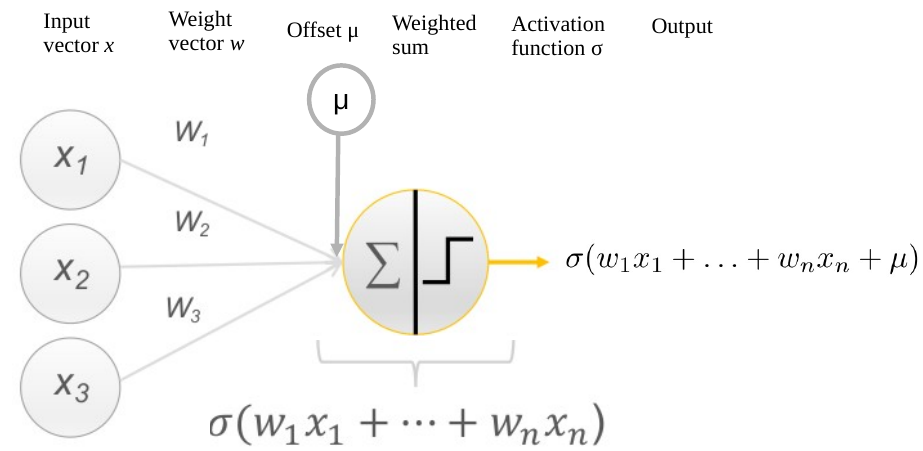
\includegraphics[scale=0.3]{images/artN/artn1.png}
    \caption{Structure of an artificial neuron}
    \label{fig:enter-label}
\end{figure}

\begin{figure}
    \centering
    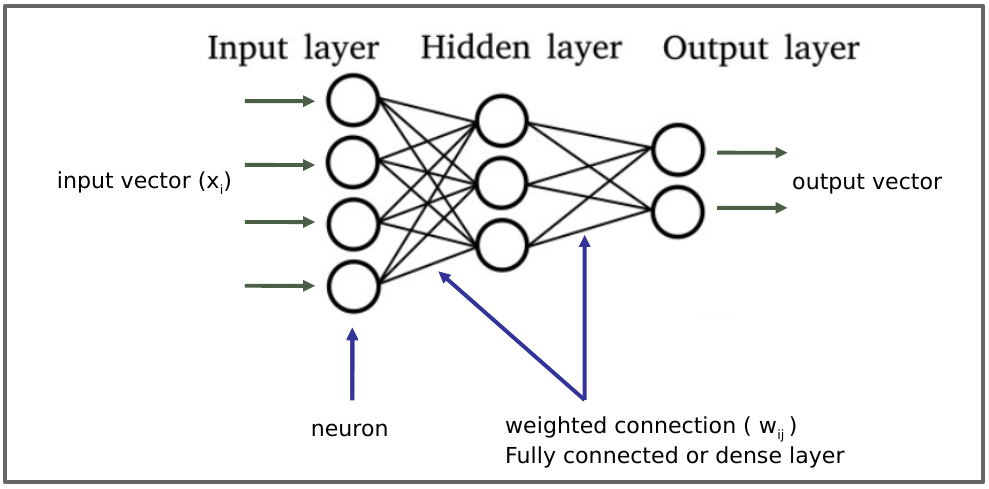
\includegraphics[scale=0.3]{images/artN/artn2.png}
    \caption{Neural network schema}
    \label{fig:enter-label}
\end{figure}

In order to train a NN
\begin{enumerate}
    \item For each neuron, definition of
    \begin{itemize}
        \item set of weights
        \item offset value 
    \end{itemize}
    \item  Define a loss function to have an empirical error over a training set
    \item  Iterative approach on training data instances to solve ERM
    \item Backpropagation of errors with gradient descent algorithm
\end{enumerate}

\begin{figure}[H]
    \centering
    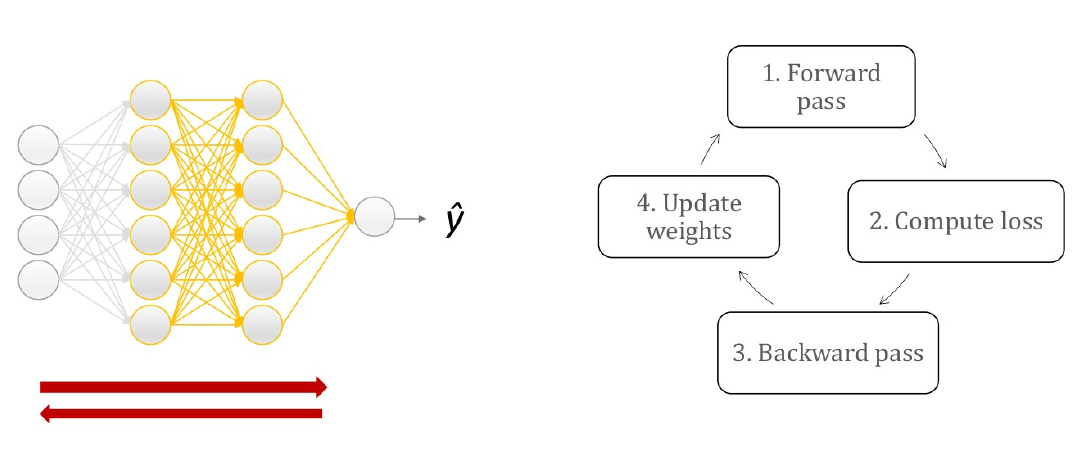
\includegraphics[scale=0.3]{images/artN/artn3.png}
    \caption{process for gradient descent algorithm}
    \label{fig:enter-label}
\end{figure}
 The process can end if \% of loss below a given threshold (or metric above given threshold) or \% of parameter variation below a given threshold or if The maximum number of epochs is reached.
 \section{Gradient descent step}
 For first thing we have to compute the forward pass.
 \begin{figure}[H]
     \centering
     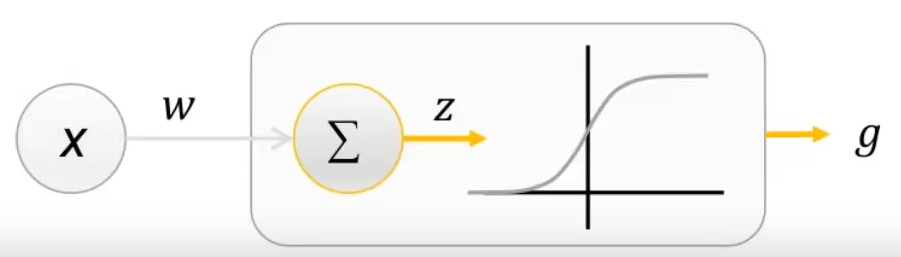
\includegraphics[scale=0.3]{images/artN/artn4.png}
     \caption{Pass to have a result}
     \label{fig:enter-label}
 \end{figure}
Forward pass:
$z = wx$ and $g= \dfrac{1}{1+e^{-z}}$. Loss is $L= -y ln(g) - (1 -y) ln(1-g)$.\\
The $g$ is an activation function like a sigmoid and $\sum$ is a multiplication. The loss function use only y and g and if y and g are similar the loss tend to 0, if different the result tend to an high number. All we can modify is w to have better results.\\
Backward pass: 
We can rewrite $-y ln(g)$ as $ \dfrac{\partial L(w)}{\partial w} $. Now for some good properties we have $\dfrac{\partial L(w)}{\partial w} = \dfrac{\partial L}{\partial g} \times \dfrac{\partial g}{\partial z} \times \dfrac{\partial z}{\partial w}$.\\
Full gradient: $ \nabla L(w) = \dfrac{\partial L}{\partial w} = \dfrac{\partial L}{\partial g} \times \dfrac{\partial g}{\partial z} \times \dfrac{\partial z}{\partial w}$.\\
this local gradient are simple to compute $\dfrac{\partial z}{\partial w} = x $ and $ \dfrac{\partial g}{\partial z} = g(1-g) $ and $\dfrac{\partial L}{\partial g} = - \dfrac{y}{g}+ \dfrac{1-y}{1-g} $.\\

Gradient step : $ w^{(k+1)} = w^{(k)}  - \alpha \nabla f(w^{(k)})$.\\

 All this is for one neurons, for more neurons we have to adding components to the chain rule using the chain rule above.
 The hyperparameter to set are the learning rate $\alpha$, the epochs the batch size and the version of the optimizer.

 The biggest problem with neural networks is the output of the neuron that, if there is not an activation function is only linear.
 So to provide non linearity we have to use activation functions to the computation. Some example are:
 \begin{itemize}
     \item Sigmoid : $\dfrac{1}{1+ e^{-x}}$
     \item Tanh: $\dfrac{e^{x}- e^{-x}}{e^x + e^{-x}} $
     \item Binary step: $ H(x) := \begin{cases}
                1, & x \ge 0 \\
                0 & x<0
                \end{cases}$
    \item ReLU (Rectified Linear Unit) neuron activate only for positive input: = $\begin{cases}
        0 & x \leq 0 \\
        x & x>0
    \end{cases}$
     \item Softmax: consider all the neurons in the output layer and the output is a probability for the input patter of belonging to each class. $Softmax(z_j) = \dfrac{e^{z_j}}{\sum\limits_{i=0}^{N-1}e^{z_j} }$
 \end{itemize}

 
 \begin{table}[H]
     \centering
     \begin{tabular}{ccc}
         Problem type & Last layer activation & Loss function\\ \hline
         Binary classification & sigmoid & Binary\_crossentropy\\ 
         Multiclass, single-label classification & softmax & categorical\_crossentropy \\ 
         Multiclass, multilabel classification & sigmoid & binary\_crossentropy\\ 
         Regression to arbitrary values & None & mse \\ 
         Regression to values between 0 and 1 & sigmoid & mse or binary\_crossentropy\\ 
     \end{tabular}
     \caption{Choosing the right last layer activastion}
     \label{tab:my_label}
 \end{table}

 The issue on using Artificial neural networks is the long training time, the coplex configuration and the fact that are black box model.
 Other example are: 
 \begin{itemize}
     \item Autoencoders
     \item Recurrent Neural Networks
     \item Convolutional neural networks
     \item Word embeddings
 \end{itemize}